%-----------------------------------------------------------------------------------------------%
%
% Maret 2019
% Template Latex untuk Tugas Akhir Program Studi Sistem informasi ini
% dikembangkan oleh Inggih Permana (inggihjava@gmail.com)
%
% Template ini dikembangkan dari template yang dibuat oleh Andreas Febrian (Fasilkom UI 2003).
%
% Orang yang cerdas adalah orang yang paling banyak mengingat kematian.
%
%-----------------------------------------------------------------------------------------------%

%-----------------------------------------------------------------------------%
\chapter{\babLima}

\section{Implementasi Sistem}
Implementasi sistem merupakan tahap dimana sistem yang telah dirancang akan dijalankan. Implementasi sistem ini meliputi implementasi \textit{database}, implementasi \textit{routes}, implementasi \textit{model}, implementasi \textit{view}, dan implementasi \textit{controller}. Implementasi sistem ini dilakukan dengan menggabungkan 2 \textit{framework} yaitu Laravel dan Codeigniter.

\subsection{Batasan Implementasi}
Batasan implementasi Sistem Informasi Inventaris Laboratorium (SITARIS) dalam penelitian untuk Kerja Praktek ini adalah:
\begin{enumerate}
	\item Sistem yang dibangun memiliki \textit{platform} berbasis\textit{ Web}.
	\item Sistem yang dibangun memiliki hak akses seperti Admin, Kalab, Kaprodi, Sekprodi, dan Aslab.
	\item Menggunakan bahasa pemrograman PHP dengan \textit{Framework} CodeIgniter dan \textit{Database} MariaDB/PHPMyadmin.
	\item Sistem dapat menampilkan data barang, pendanaan, dokumentasi, peminjaman barang, peminjaman ruangan, \textit{maintenance}, pemusnahan barang, fakultas/lembaga, program studi/unit, gedung, ruangan, jadwal, dosen, mata kuliah dan pengguna.
\end{enumerate}

\subsection{Implementasi Perangkat Keras (\textit{Hardware})}
% -----------------------------------------------------------------------------%
Implementasi pada lingkungan \textit{hardware} adalah implementasi pada perangkat keras yang digunakan untuk menjalankan sistem informasi manajemen laboratorium. Implementasi \textit{hardware} yang digunakan dapat dilihat pada Tabel 5.1.

Minimum kebutuhan pada implementasi \textit{hardware} untuk menjalankan sistem informasi manajemen laboratorium adalah spesifikasi perangkat keras yang harus terpenuhi agar sistem dapat beroperasi secara optimal. Tabel 5.1. menyajikan daftar rinci dari komponen perangkat keras yang diperlukan dan spesifikasinya yang mencakup prosesor, RAM, Hardisk, Monitor, dan perangkat masukan yang harus memenuhi standar minimum agar sistem berfungsi dengan baik.

\begin{longtable}{l l}
	\caption{Spesifikasi Perangkat Keras (\textit{Hardware})}                                                               \\
	\hline
	\textbf{ Komponen \textit{Hardware}} & \textbf{ Spesifikasi}                                                            \\
	\hline
	\endfirsthead

	\multicolumn{2}{c}{\tablename\ \thetable\ {Spesifikasi Perangkat Keras (\textit{Hardware})} \space (Tabel lanjutan...)} \\
	\hline
	\textbf{ Komponen \textit{Hardware}} & \textbf{ Spesifikasi}                                                            \\
	\hline
	\endhead

	Processor                            & Intel \textregistered{} CoreTM i3-4160, 3.60GHz                                  \\
	Memory (RAM)                         & 2 GB                                                                             \\
	Hardisk (HDD)                        & 1 TB                                                                             \\
	LCD                                  & Lenovo 17"                                                                       \\
	\hline
\end{longtable}

\subsection{Implementasi Perangkat Lunak (\textit{Software})}
% -----------------------------------------------------------------------------%
Implementasi pada lingkungan \textit{software} adalah implementasi pada perangkat lunak yang digunakan untuk menjalankan sistem informasi inventaris laboratorium. Implementasi \textit{software} yang digunakan dapat dilihat pada Tabel 5.2.

\begin{longtable}{l l}
	\caption{Spesifikasi Perangkat Lunak (\textit{Software})}                                                               \\
	\hline
	\textbf{ Komponen \textit{Software}} & \textbf{ Spesifikasi}                                                            \\
	\hline
	\endfirsthead

	\multicolumn{2}{c}{\tablename\ \thetable\ {Spesifikasi Perangkat Lunak (\textit{Software})} \space (Tabel lanjutan...)} \\
	\hline
	\textbf{ Komponen \textit{Software}} & \textbf{ Spesifikasi}                                                            \\
	\hline
	\endhead

	Sistem Operasi                       & Windows 7, 8, 10, dan 11                                                         \\
	Browser                              & Google Chrome dan Mozilla Firefox                                                \\
	Bahasa Pemrograman                   & PHP dan Javascript                                                               \\
	Web \textit{Database}                & MariaDB                                                                          \\
	\textit{Framework}                   & CodeIgniter 4                                                                    \\
	\hline
\end{longtable}

\subsection{Implementasi \textit{Database}}
Pada implementasi \textit{database} ini nama yang digunakan adalah ”man\_lab”. Implemenasi \textit{database} ini terdapat beberapa tabel yang akan digunakan dalam sistem. Pembuatan \textit{database} dilakukan dengan menggunakan \textit{database} MariaDB. Tabel-tabel ini akan digunakan untuk menyimpan data-data yang diperlukan dalam sistem. Berikut adalah struktur tabel yang telah diintegrasikan dan digunakan dalam sistem ini dapat dilihat pada Lampiran \ref{database-manlab}. Pada pengembangan kali ini dilakukan penambahan tabel baru yaitu tabel "jadwal", "dosen", "mata kuliah", dan tabel  "biodatas", "users", "kelola pendaftarans", "kelola ujians", "postingans", "soals", jawabans", dan "wawancaras" sebagai tabel tambahan untuk integrasi sistem.

\begin{enumerate}

	\item Tabel Dosen dirancang untuk menyimpan informasi penting terkait dosen dalam sebuah sistem informasi. Kolom id\_dosen berfungsi sebagai kunci utama (primary key) yang memastikan setiap data dosen bersifat unik dan tidak terjadi duplikasi. Kolom nama\_dosen digunakan untuk mencatat nama lengkap dosen, sedangkan nip\_dosen menyimpan Nomor Induk Pegawai (NIP) sebagai identitas resmi dosen, jika tersedia. Untuk mencatat jenis kelamin, digunakan kolom jenis\_kelamin dengan opsi seperti "Laki-laki" atau "Perempuan". Informasi kontak dosen dicatat melalui kolom email\_dosen dan no\_hp yang masing-masing menyimpan alamat email serta nomor handphone. Selain itu, kolom nidn digunakan untuk menyimpan Nomor Induk Dosen Nasional (NIDN) sebagai identitas unik dosen di tingkat nasional. Semua kolom ini dirancang untuk memastikan data dosen tersimpan secara lengkap, terstruktur, dan mudah diakses. Tampilan dapat dilihat pada Gambar \ref{tabel-Dosen}.

	      \begin{figure}
		      \centering
		      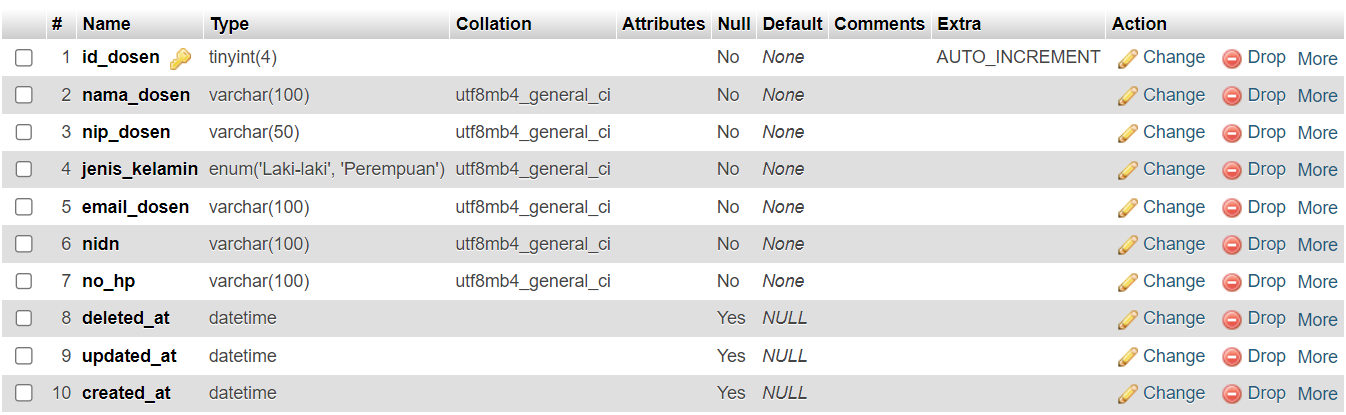
\includegraphics[width=0.82\textwidth]{konten/gambar/implementasi/tabel-dosen.png}
		      \caption{Tampilan \textit{Database} Tabel Dosen}
		      \label{tabel-Dosen}
	      \end{figure}


	\item Tabel Matkul digunakan untuk menyimpan informasi mengenai mata kuliah dalam sistem informasi akademik. Kolom id\_matkul berfungsi sebagai kunci utama \textit{(primary key)} untuk mengidentifikasi setiap mata kuliah secara unik dan mencegah terjadinya duplikasi data. Kolom kode\_matkul menyimpan kode unik mata kuliah sebagai referensi singkat. Nama mata kuliah dicatat dalam kolom nama\_matkul untuk memberikan informasi deskriptif terkait mata kuliah tersebut. Kolom sks digunakan untuk mencatat jumlah Sistem Kredit Semester (SKS) dari mata kuliah, sedangkan semester mencatat pada semester berapa mata kuliah tersebut ditawarkan. Selain itu, kolom jenis\_matkul digunakan untuk mengklasifikasikan jenis mata kuliah, misalnya wajib dan pilihan. Struktur tabel ini dirancang untuk memastikan data terkait mata kuliah tersimpan secara terorganisasi dan mudah diakses sesuai kebutuhan. Tampilan dapat dilihat pada Gambar \ref{tabel-Matkul}.

	      \begin{figure}
		      \centering
		      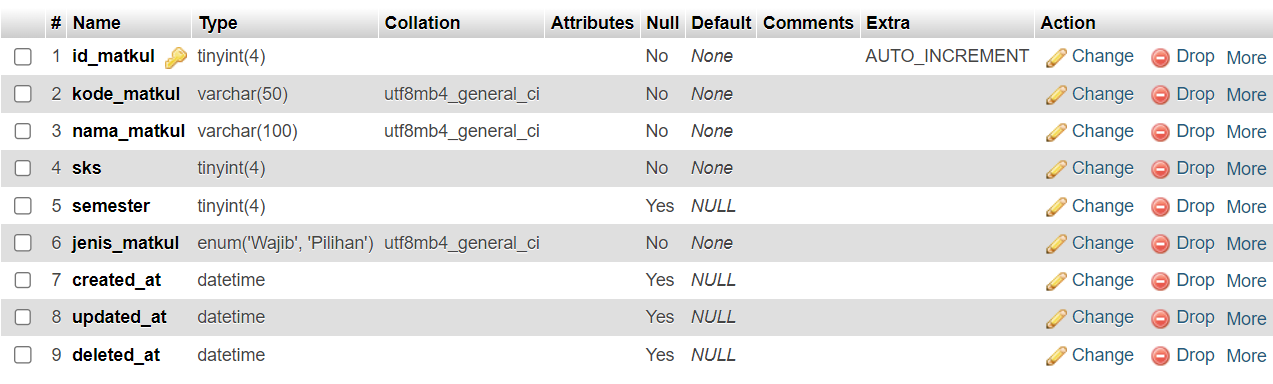
\includegraphics[width=0.82\textwidth]{konten/gambar/implementasi/tabel-matkul.png}
		      \caption{Tampilan \textit{Database} Tabel Matkul}
		      \label{tabel-Matkul}
	      \end{figure}

	\item Tabel Jadwal  terdiri dari kolom id\_jadwal yang menjadi kunci utama dari tabel tersebut yang digunakan sebagai penanda agar tidak terjadi duplikasi data, id\_ruangan digunakan untuk menunjukkan ruangan yang digunakan, id\_matkul digunakan untuk menunjukkan mata kuliah yang digunakan, id\_dosen digunakan untuk menunjukkan dosen yang mengajar, tanggal digunakan untuk menunjukkan tanggal pelaksanaan, hari digunakan untuk menunjukkan hari laboratorium digunakan, jam\_masuk dan jam\_keluar digunakan untuk menunjukkan jam digunakannya laboratorium, dan deskripsi digunakan untuk menunjukkan deskripsi dari jadwal tersebut. Tampilan dapat dilihat pada Gambar \ref{tabel-jadwal}.

	      \begin{figure}
		      \centering
		      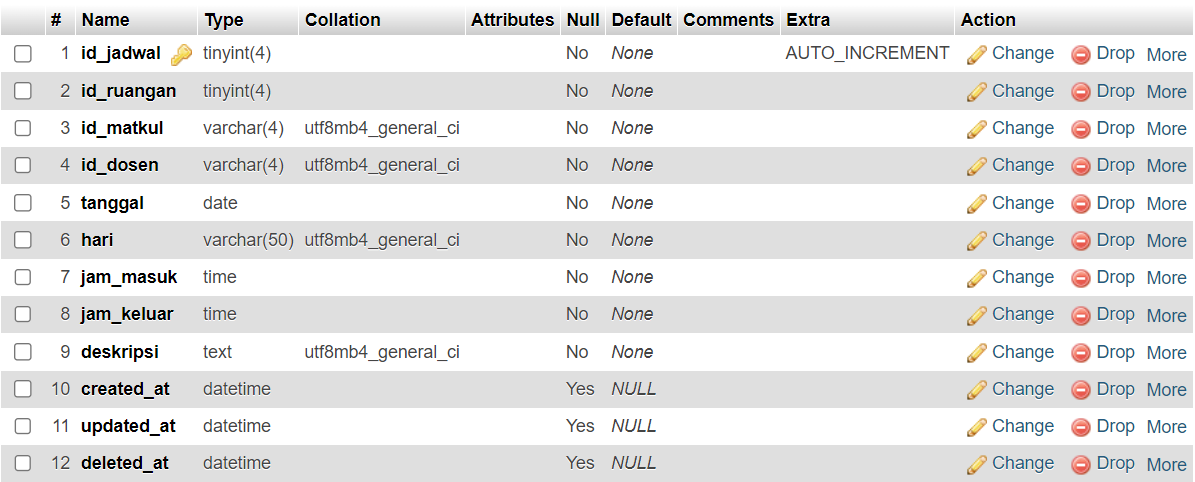
\includegraphics[width=0.82\textwidth]{konten/gambar/implementasi/tabel-jadwal.png}
		      \caption{Tampilan \textit{Database} Tabel Jadwal}
		      \label{tabel-jadwal}
	      \end{figure}

	\item Tabel Ruangan terdiri dari kolom id\_ruangan yang menjadi kunci utama dari tabel tersebut yang digunakan sebagai penanda agar tidak terjadi duplikasi data, id\_gedung menjadi kunci asing dalam tabel ruangan karena nama gedung diperlukan dalam pencatatan data ruangan, nama\_ruangan adalah kolom yang menyimpan nama ruangan yang dicatat, deskripsi\_ruangan menjelaskan detail tentang ruangan yang dicatat, gambar\_ruangan merupakan kolom untuk menyimpan data gambar dari ruangan yang dicatat. Tampilan dapat dilihat pada Gambar \ref{fig:tabel-ruangan}.

	      \begin{figure}
		      \centering
		      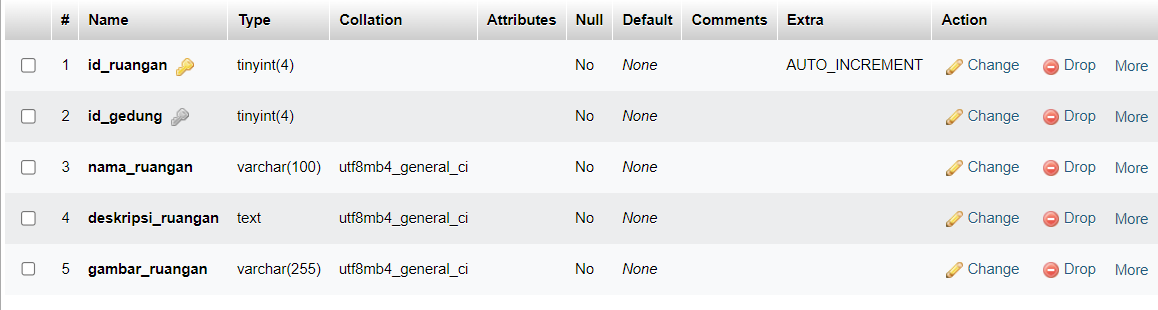
\includegraphics[width=0.82\linewidth]{konten//gambar/Tampilan database tabel ruangan.png}
		      \caption{Tampilan \textit{Database} Tabel Ruangan}
		      \label{fig:tabel-ruangan}
	      \end{figure}

	\item Tabel User terdiri dari kolom id\_user yang menjadi kunci utama dari tabel tersebut yang digunakan sebagai penanda agar tidak terjadi duplikasi data, nama merupakan kolom yang menyimpan nama pengguna, foto merupakan kolom untuk menyimpan foto profil pengguna, no\_identitas merupakan kolom yang digunakan untuk menyimpan data NIM, NIP, atau NIK dari pengguna, \textit{username} merupakan kolom yang digunakan untuk menyimpan \textit{username} pengguna, password\_hash merupakan kolom yang digunakan untuk menyimpan \textit{password} pengguna, email merupakan kolom yang digunakan untuk menyimpan email pengguna, role\_user merupakan kolom yang digunakan untuk menyimpan level akses pengguna. Tampilan dapat dilihat pada Gambar \ref{fig:tabel-user}.

	      \begin{figure}
		      \centering
		      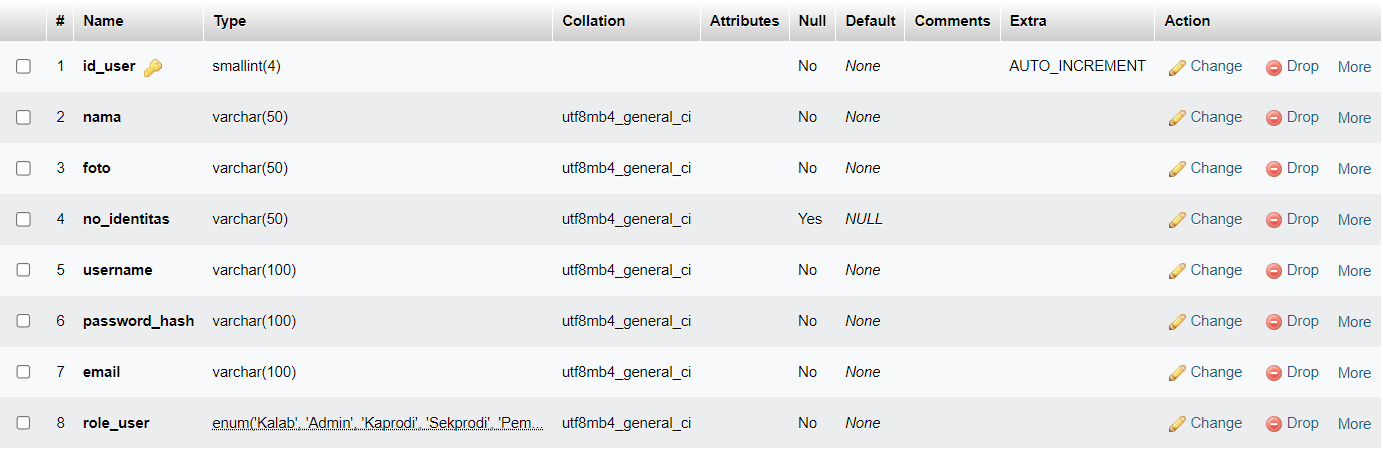
\includegraphics[width=0.82\linewidth]{konten//gambar/Tampilan database tabel user.png}
		      \caption{Tampilan \textit{Database} Tabel \textit{User}}
		      \label{fig:tabel-user}
	      \end{figure}
\end{enumerate}

\subsection{Implementasi \textit{Routes}}
\textit{Routes} dalam konsep \textit{Model View Controller} (MVC) adalah mekanisme yang digunakan untuk mengatur bagaimana permintaan \textit{(requests)} dari pengguna atau \textit{client} akan ditangani oleh aplikasi web. \textit{Routes} menentukan hubungan antara URL yang diminta oleh pengguna dengan controller yang akan menangani permintaan tersebut \cite{kelvin2022sistem}. Dalam pengembangan ini ditambahkan beberapa \textit{routes} untuk menangani \textit{requests} pada sistem informasi.

\begin{enumerate}
	\item \textit{Routes} dalam implementasi Sistem Manajemen Laboratorium pada data dosen dapat dilihat pada Gambar \ref{fig:routes-dosen}
	      \begin{figure}
		      \centering
		      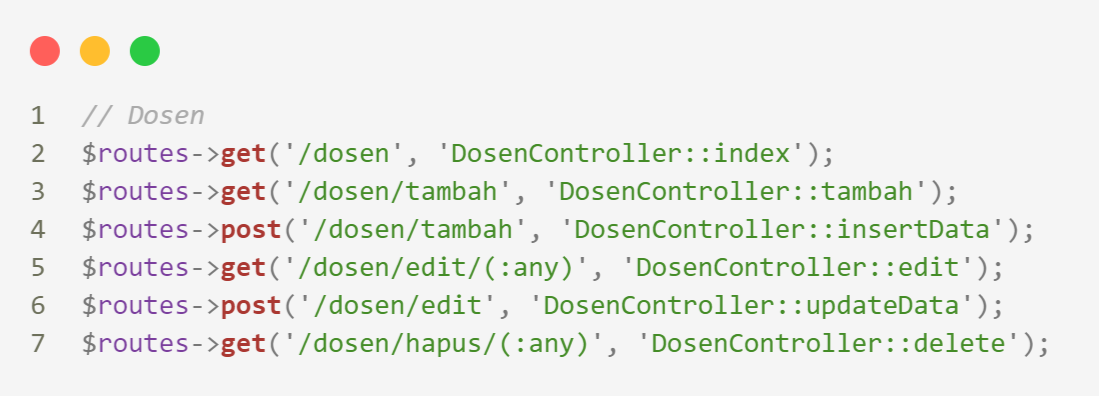
\includegraphics[width=0.82\linewidth]{konten//gambar/routes/dosen.png}
		      \caption{Tampilan \textit{Routes} Dosen}
		      \label{fig:routes-dosen}
	      \end{figure}
	\item \textit{Routes} dalam implementasi Sistem Manajemen Laboratorium pada data matkul dapat dilihat pada Gambar \ref{fig:routes-matkul}
	      \begin{figure}
		      \centering
		      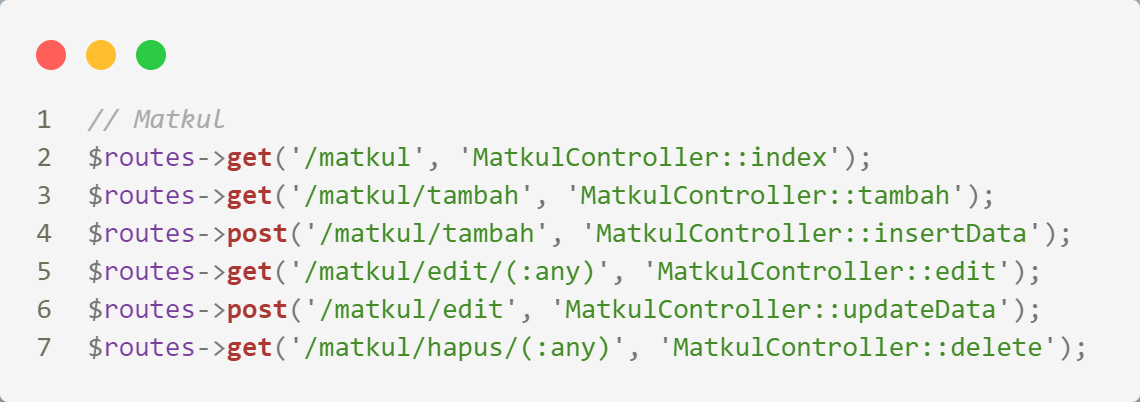
\includegraphics[width=0.82\linewidth]{konten//gambar/routes/matkul.png}
		      \caption{Tampilan \textit{Routes} Matkul}
		      \label{fig:routes-matkul}
	      \end{figure}
	\item \textit{Routes} dalam implementasi Sistem Manajemen Laboratorium pada data jadwal dapat dilihat pada Gambar \ref{fig:routes-jadwal}
	      \begin{figure}
		      \centering
		      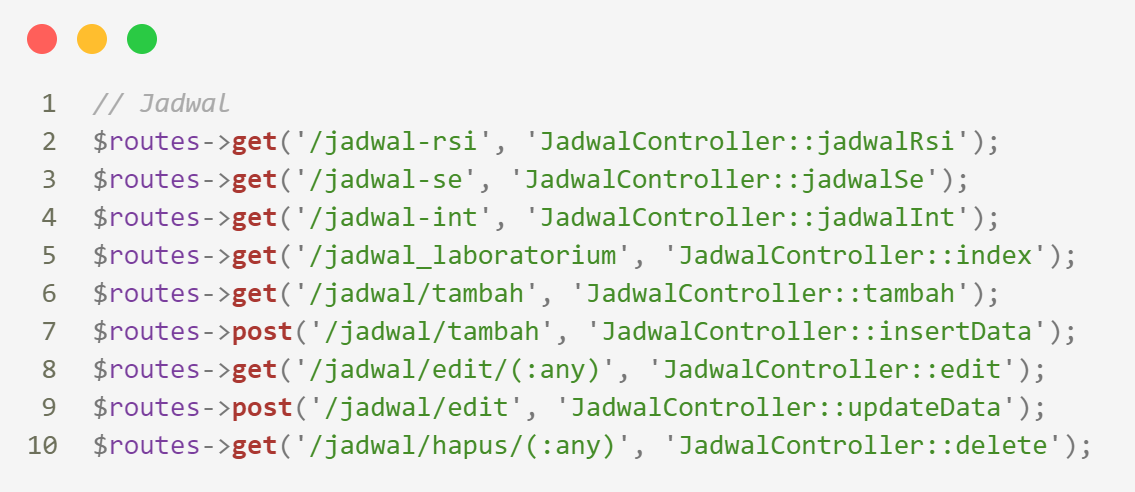
\includegraphics[width=0.82\linewidth]{konten//gambar/routes/jadwal.png}
		      \caption{Tampilan \textit{Routes} Jadwal}
		      \label{fig:routes-jadwal}
	      \end{figure}
	\item \textit{Routes} dalam implementasi Sistem Manajemen Laboratorium pada data ruangan dapat dilihat pada Gambar \ref{fig:routes-ruangan}
	      \begin{figure}
		      \centering
		      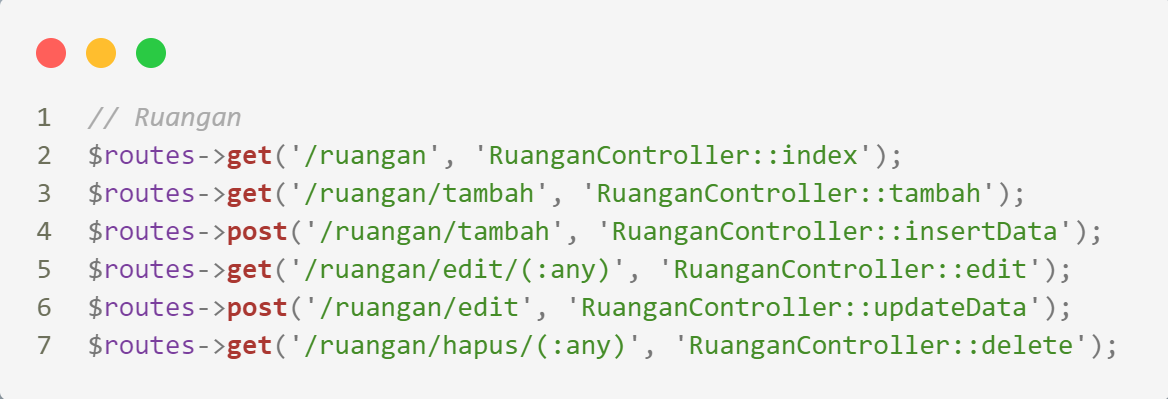
\includegraphics[width=0.82\linewidth]{konten//gambar/routes/ruangan.png}
		      \caption{Tampilan \textit{Routes} Ruangan}
		      \label{fig:routes-ruangan}
	      \end{figure}
	\item \textit{Routes} dalam implementasi Sistem Manajemen Laboratorium pada data user dapat dilihat pada Gambar \ref{fig:routes-user}
	      \begin{figure}
		      \centering
		      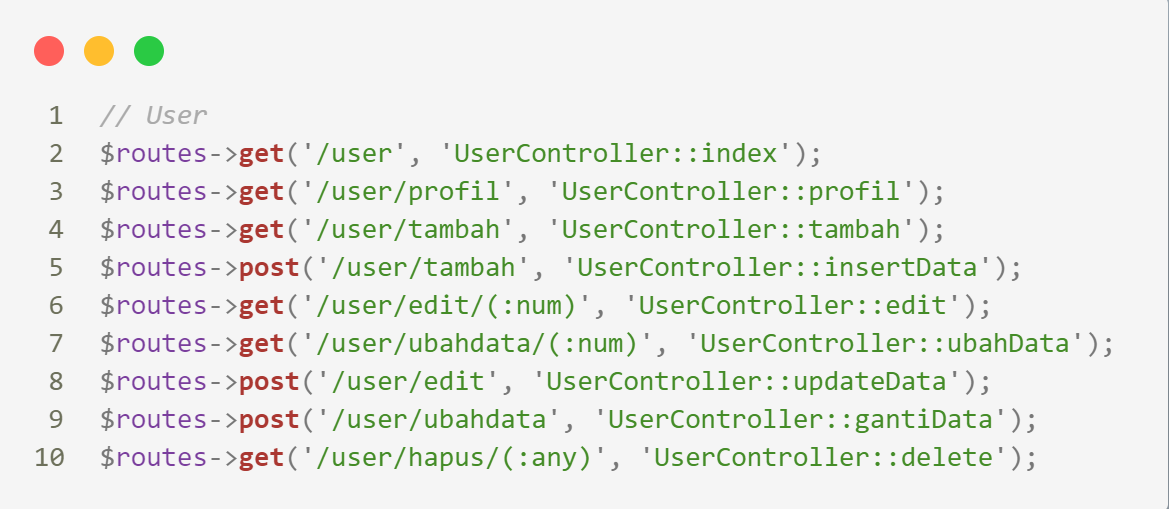
\includegraphics[width=0.82\linewidth]{konten//gambar/routes/user.png}
		      \caption{Tampilan \textit{Routes} \textit{User}}
		      \label{fig:routes-user}
	      \end{figure}
\end{enumerate}

\subsection{Implementasi \textit{Model}}
Model adalah komponen yang bertanggung jawab untuk mengatur data, aturan bisnis, dan logika aplikasi. Ini merupakan representasi dari data dalam aplikasi. Model mengelola semua operasi data, seperti pengambilan, pembaruan, dan penyimpanan data \cite{firdaus2020rancang}. Model-model ini akan diatur pada folder app/model pada \textit{Framework} CodeIgniter dapat dilihat pada Lampiran \ref{fig:implementasi-model}.



% \begin{enumerate}
% 	\item \textit{Model} dalam implementasi Sistem Manajemen Laboratorium pada data dosen dapat dilihat pada Gambar \ref{fig:model-dosen}
% 	      \begin{figure}
% 		      \centering
% 		      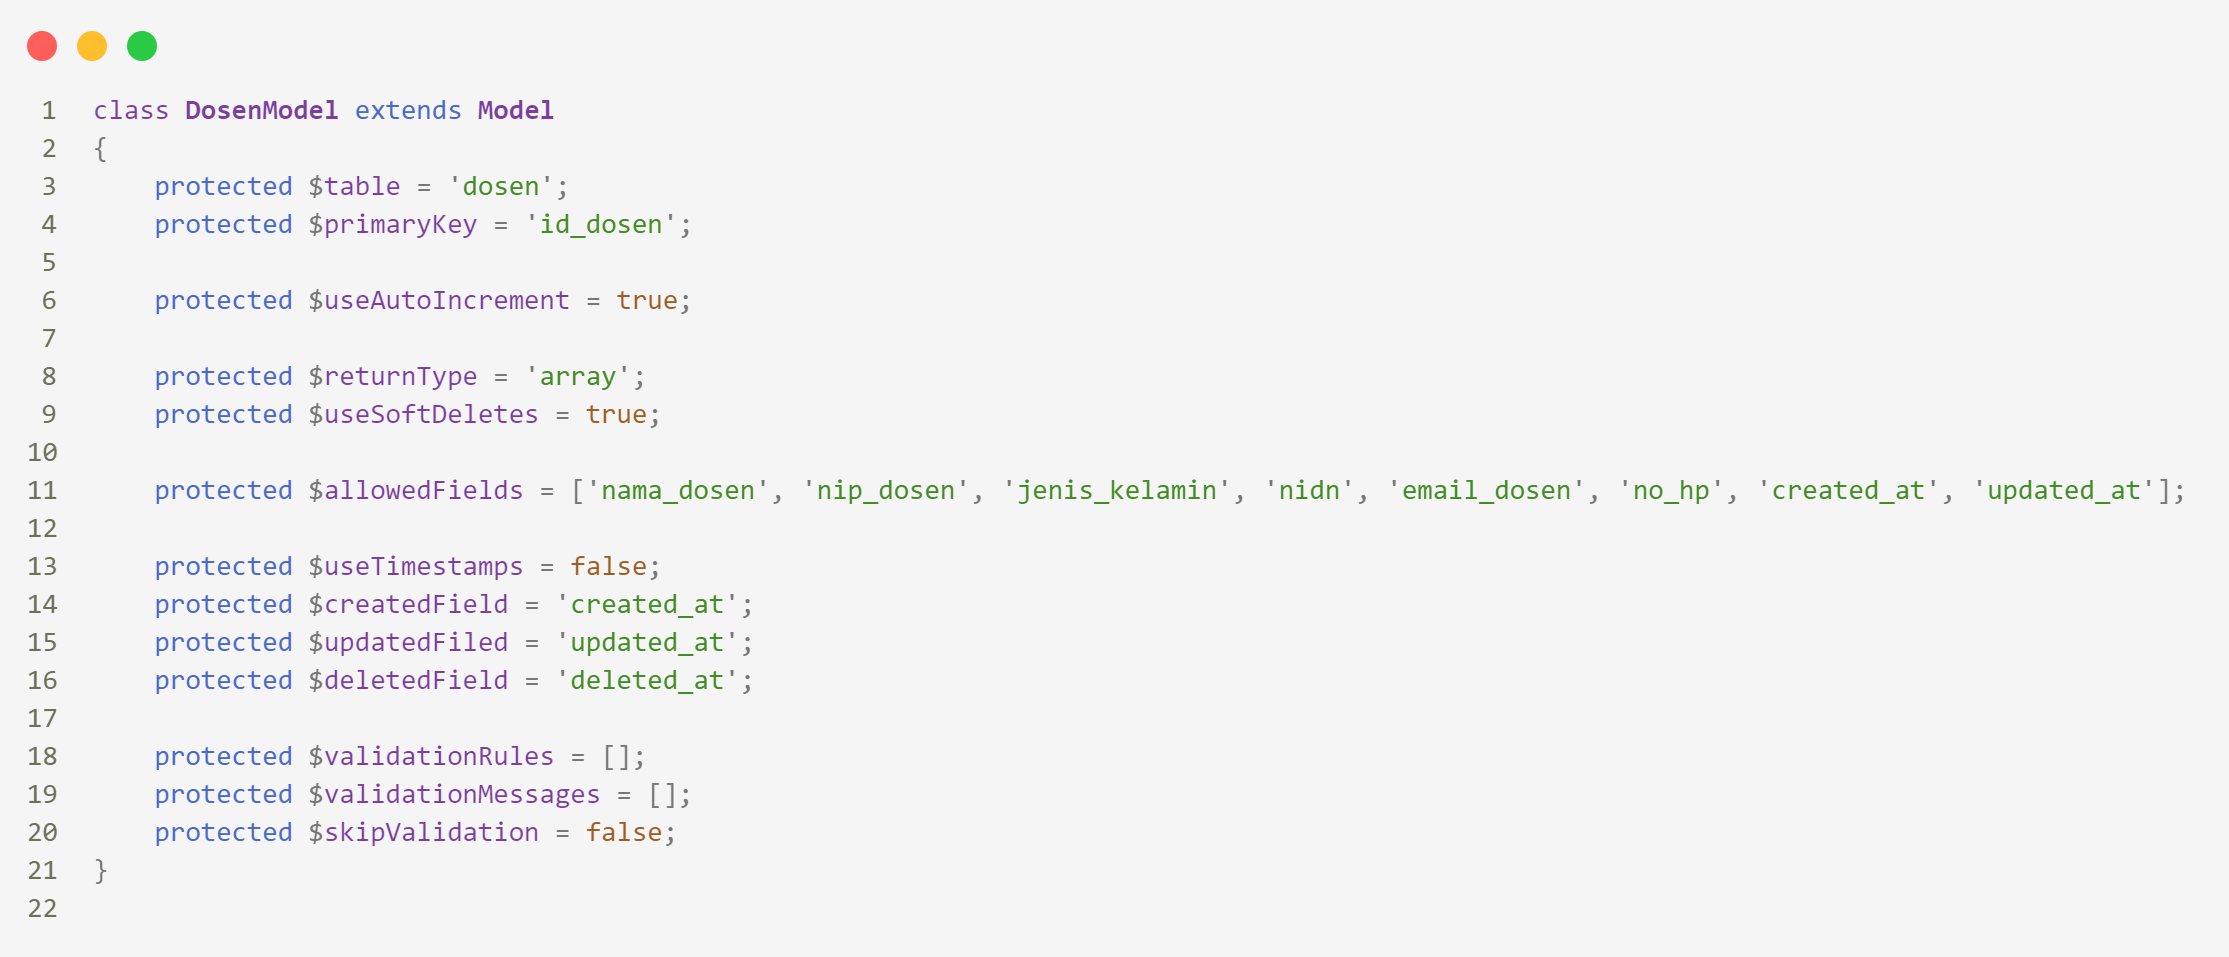
\includegraphics[width=0.82\linewidth]{konten//gambar/model/dosen.png}
% 		      \caption{Tampilan Model Dosen}
% 		      \label{fig:model-dosen}
% 	      \end{figure}
% 	\item \textit{Routes} dalam implementasi Sistem Manajemen Laboratorium pada data matkul dapat dilihat pada Gambar \ref{fig:model-matkul}
% 	      \begin{figure}
% 		      \centering
% 		      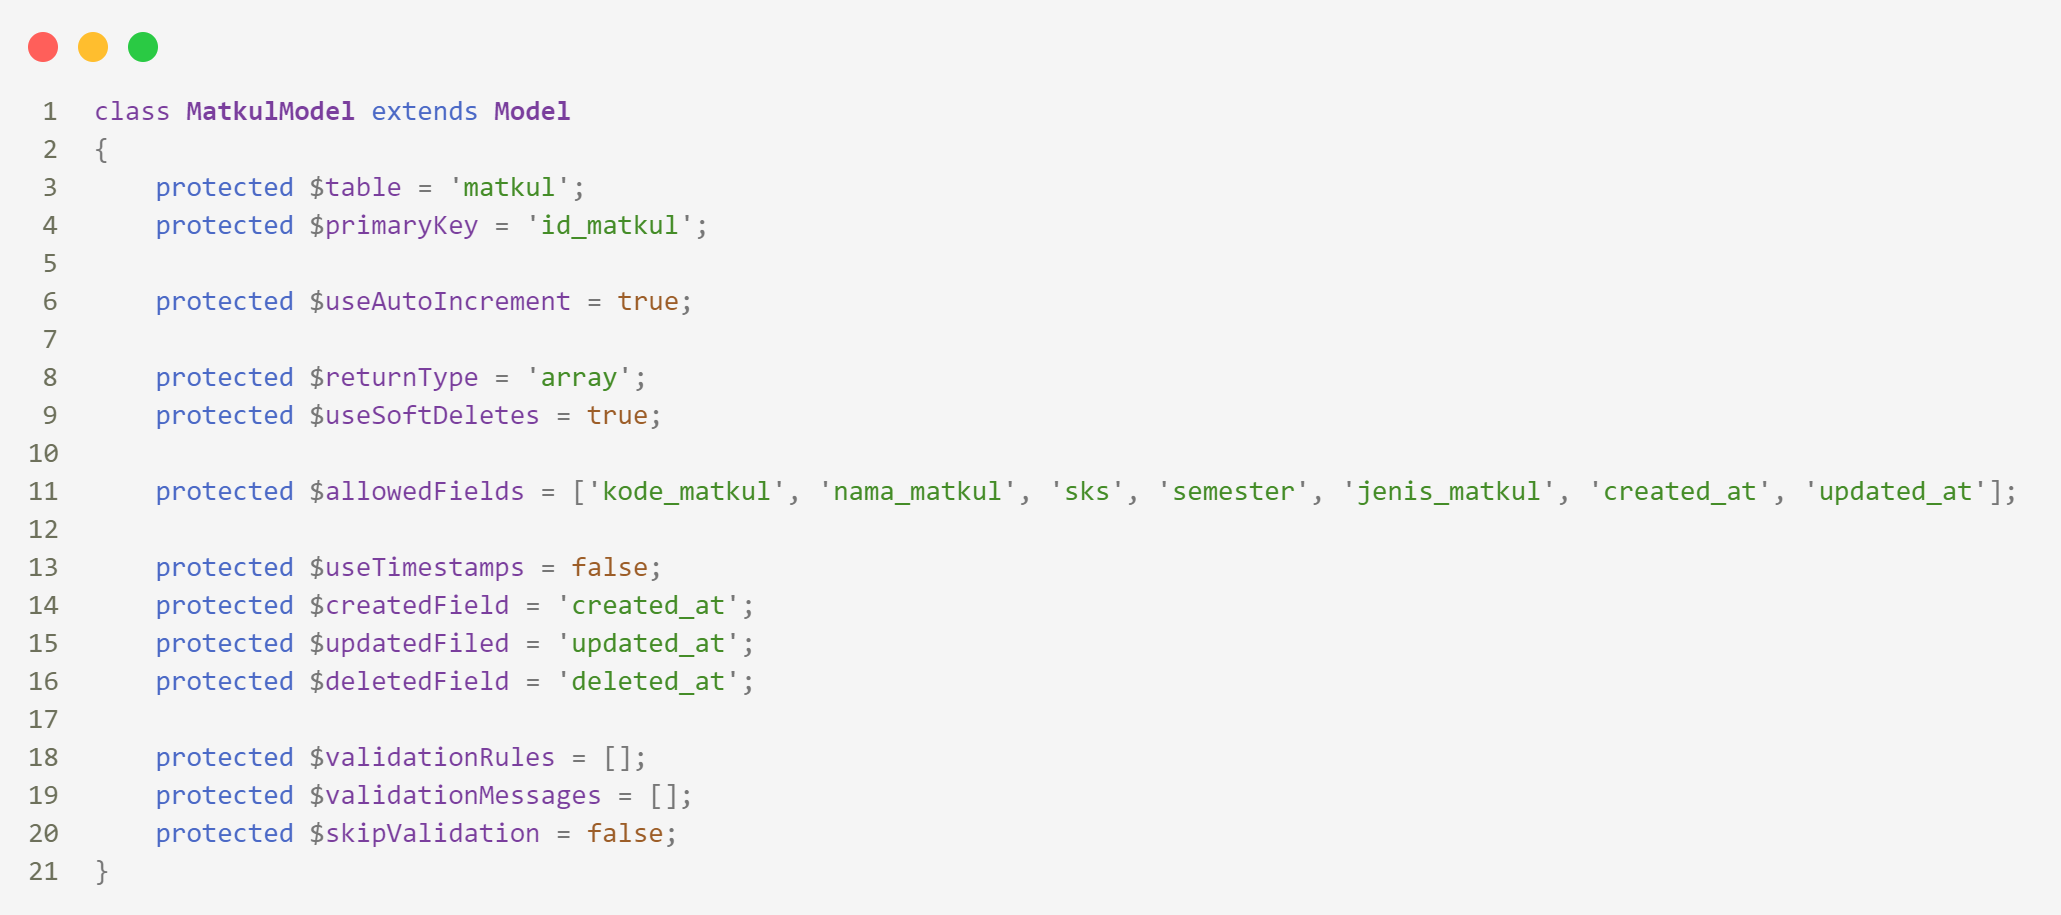
\includegraphics[width=0.82\linewidth]{konten//gambar/model/matkul.png}
% 		      \caption{Tampilan Model Matkul}
% 		      \label{fig:model-matkul}
% 	      \end{figure}
% 	\item \textit{Routes} dalam implementasi Sistem Manajemen Laboratorium pada data jadwal dapat dilihat pada Gambar \ref{fig:model-jadwal}
% 	      \begin{figure}
% 		      \centering
% 		      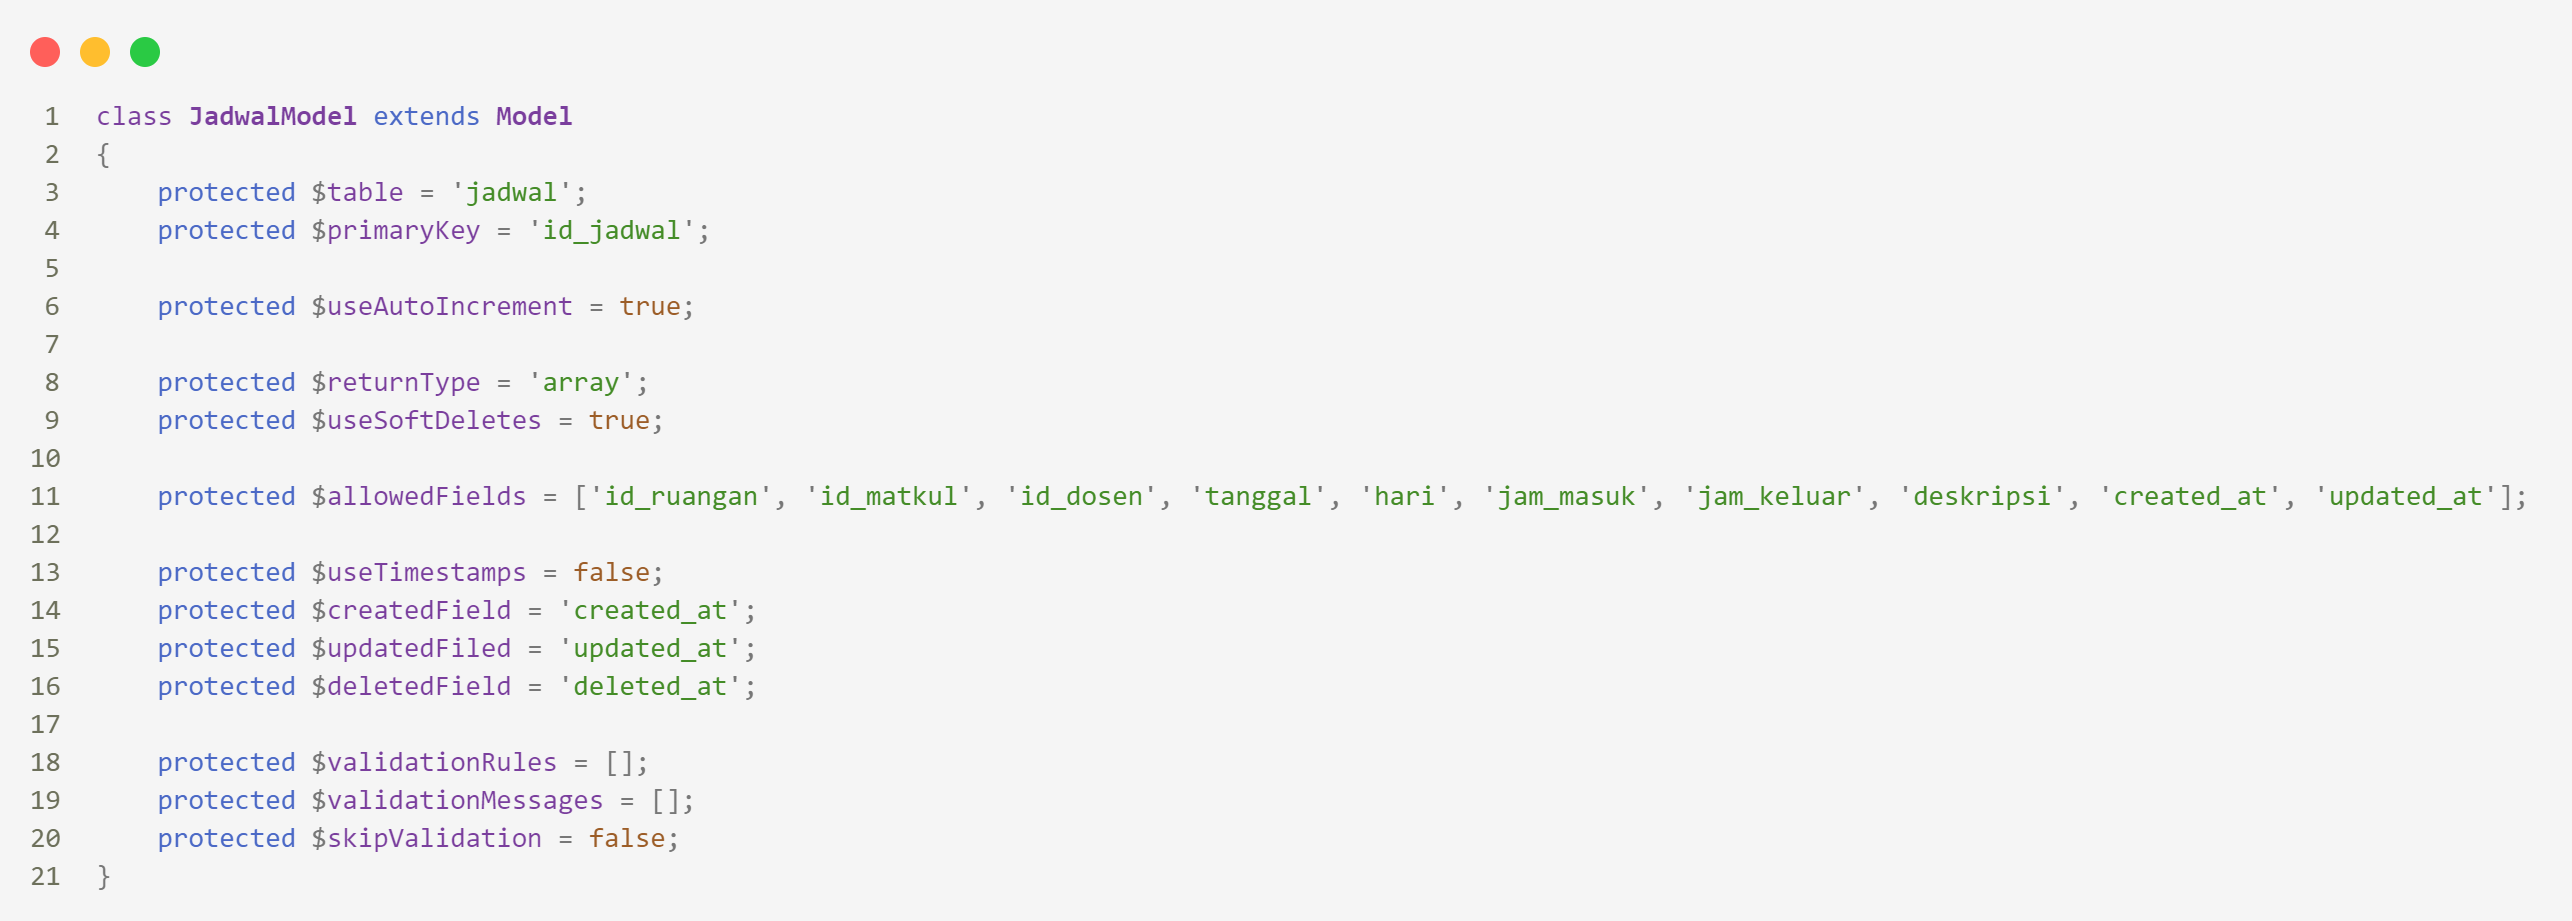
\includegraphics[width=0.82\linewidth]{konten//gambar/model/jadwal.png}
% 		      \caption{Tampilan Model Jadwal}
% 		      \label{fig:model-jadwal}
% 	      \end{figure}
% 	\item \textit{Routes} dalam implementasi Sistem Manajemen Laboratorium pada data ruangan dapat dilihat pada Gambar \ref{fig:model-ruangan}
% 	      \begin{figure}
% 		      \centering
% 		      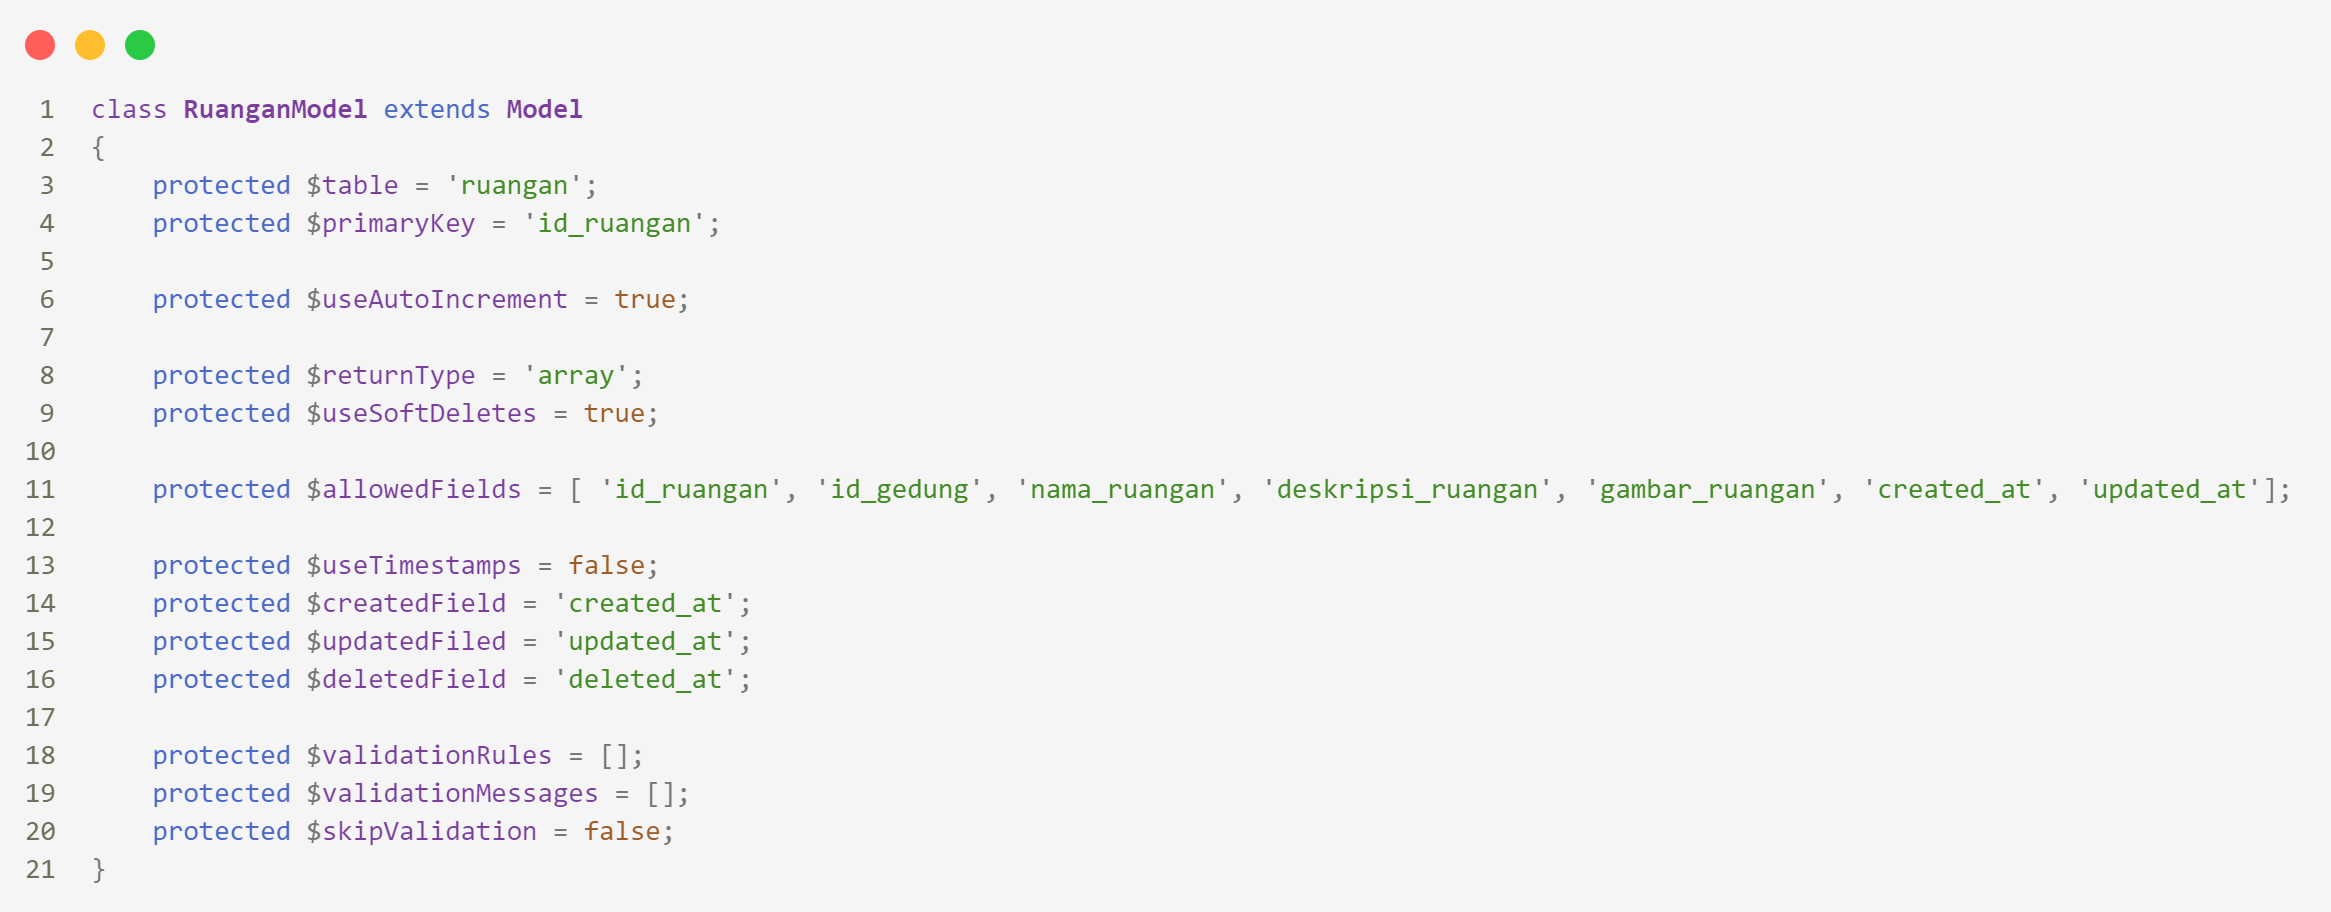
\includegraphics[width=0.82\linewidth]{konten//gambar/model/ruangan.png}
% 		      \caption{Tampilan Model Ruangan}
% 		      \label{fig:model-ruangan}
% 	      \end{figure}
% 	\item \textit{Routes} dalam implementasi Sistem Manajemen Laboratorium pada data user dapat dilihat pada Gambar \ref{fig:model-user}
% 	      \begin{figure}
% 		      \centering
% 		      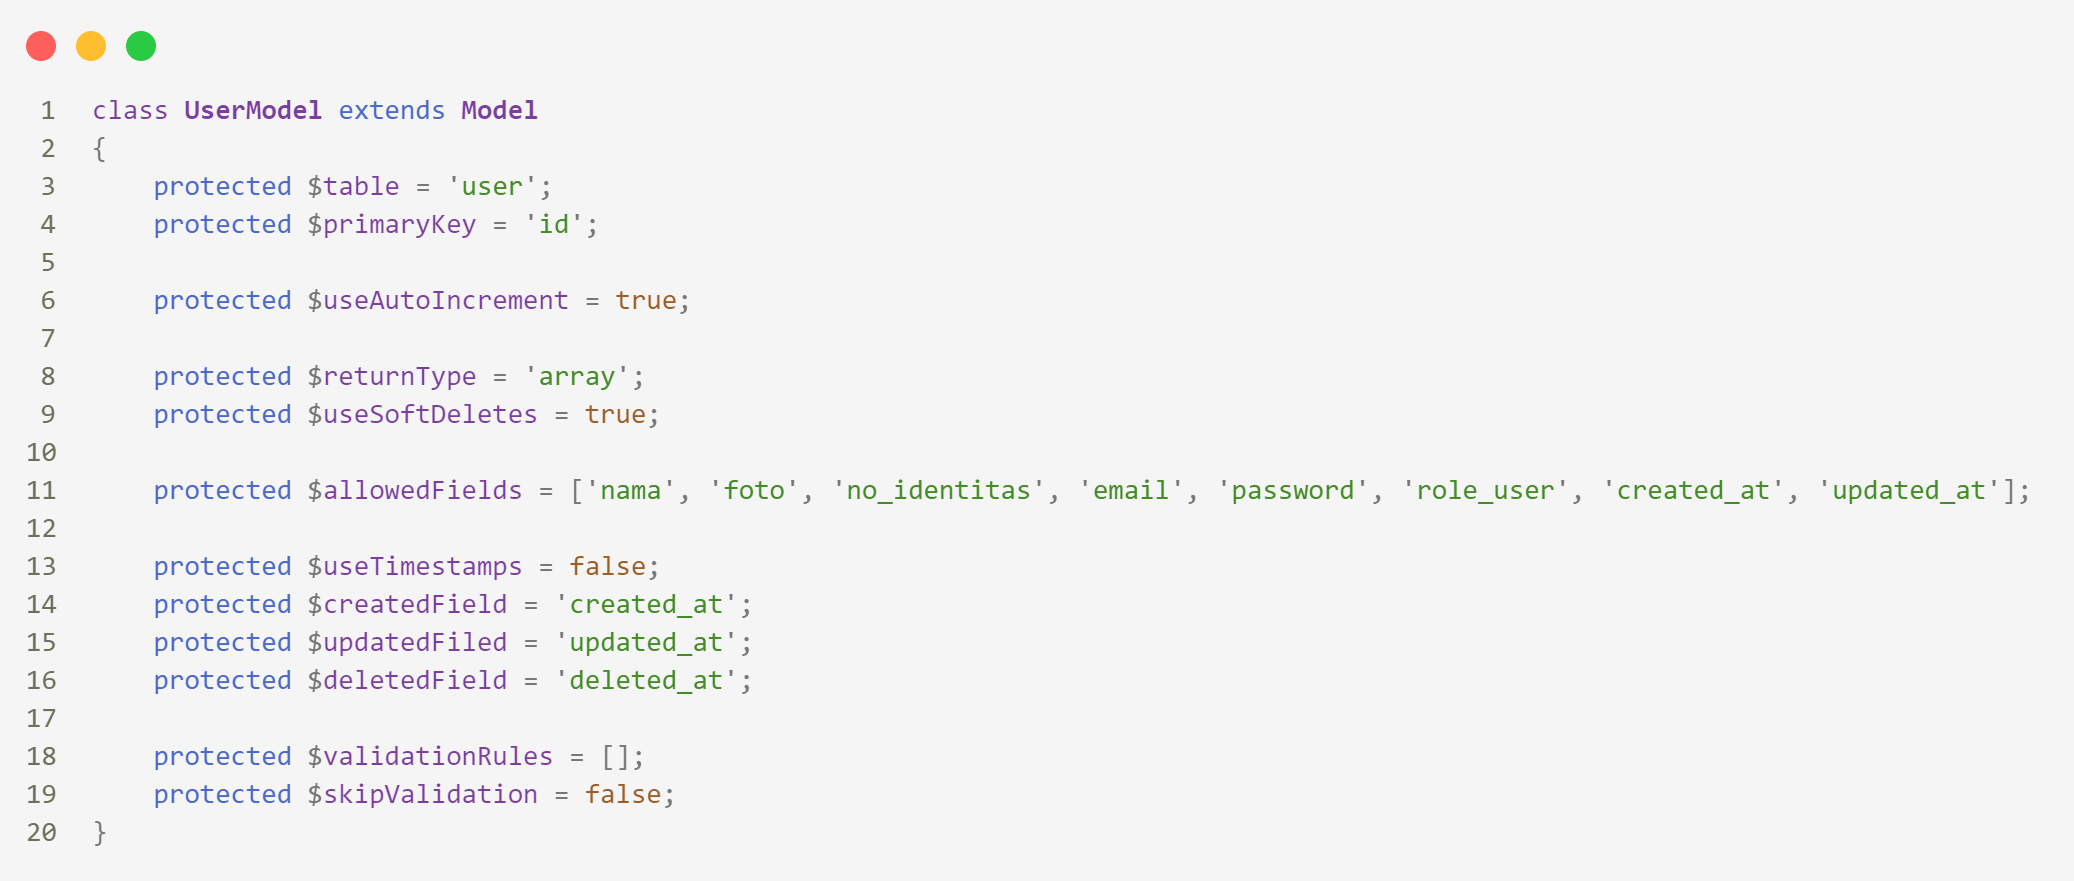
\includegraphics[width=0.82\linewidth]{konten//gambar/model/user.png}
% 		      \caption{Tampilan Model \textit{User}}
% 		      \label{fig:model-user}
% 	      \end{figure}
% \end{enumerate}

\subsection{Implementasi \textit{View}}
\textit{View }adalah komponen yang menampilkan antarmuka pengguna dan menampilkan data dari Model. \textit{View} mengamati perubahan pada Model dan \textit{Controller}, dan diperbarui sesuai keadaan terkini. Penggunaan \textit{View} memisahkan tugas penyajian dan manajemen data dalam aplikasi yang memberikan fleksibilitas dan pemeliharaan yang lebih baik \cite{firdaus2020rancang}. \textit{View} ini akan diatur pada folder app/view pada \textit{framework} CodeIgniter dapat dilihat pada Lampiran \ref{fig:implementasi-view}.

\subsection{Implementasi \textit{Controller}}
\textit{Controller} adalah komponen yang bertanggung jawab untuk mengatur logika pengendalian atau interaksi antara Model (data), \textit{View} (tampilan), dan pengguna \cite{rahman2018perancangan}. \textit{Controller} ini akan diatur pada folder app/controller pada \textit{framework} CodeIgniter dapat dilihat pada Lampiran \ref{fig:implementasi-controller}.

\subsection{Hasil Implementasi}
Beberapa permasalahan yang teridentifikasi meliputi kesalahan dalam pembuatan kode barang (Lampiran B), disfungsi fitur peminjaman barang dan ruangan (Lampiran B), serta ketidaksesuaian format laporan akhir dengan kebutuhan kepala laboratorium (Lampiran B). Kesalahan dalam pembuatan kode barang menyebabkan ketidakakuratan dalam pencatatan dan pelacakan inventaris yang dapat mengakibatkan kesulitan dalam manajemen barang. Disfungsi fitur peminjaman barang dan ruangan menghambat proses peminjaman yang seharusnya berjalan lancar, sehingga pengguna mengalami kesulitan dalam meminjam barang dan ruangan yang dibutuhkan. Ketidaksesuaian format laporan akhir dengan kebutuhan kepala laboratorium menyebabkan informasi yang disampaikan tidak sesuai dengan yang diharapkan, sehingga memerlukan penyesuaian agar laporan lebih relevan dan mudah dipahami. Saya sudah memperbaiki kesalahan ini dengan melakukan beberapa perubahan dan penyesuaian pada sistem. Hasil dari perbaikan tersebut akan saya tampilkan untuk menunjukkan peningkatan yang telah dicapai.

\begin{enumerate}
	\item Tampilan kode barang yang berfungsi untuk memberikan informasi mengenai kode barang dalam sistem manajemen laboratorium. Halaman ini memberikan gambaran umum tentang pengelolaan kode barang. Dapat dilihat pada Gambar \ref{fig:kode-barang}.
	      \begin{figure}
		      \centering
		      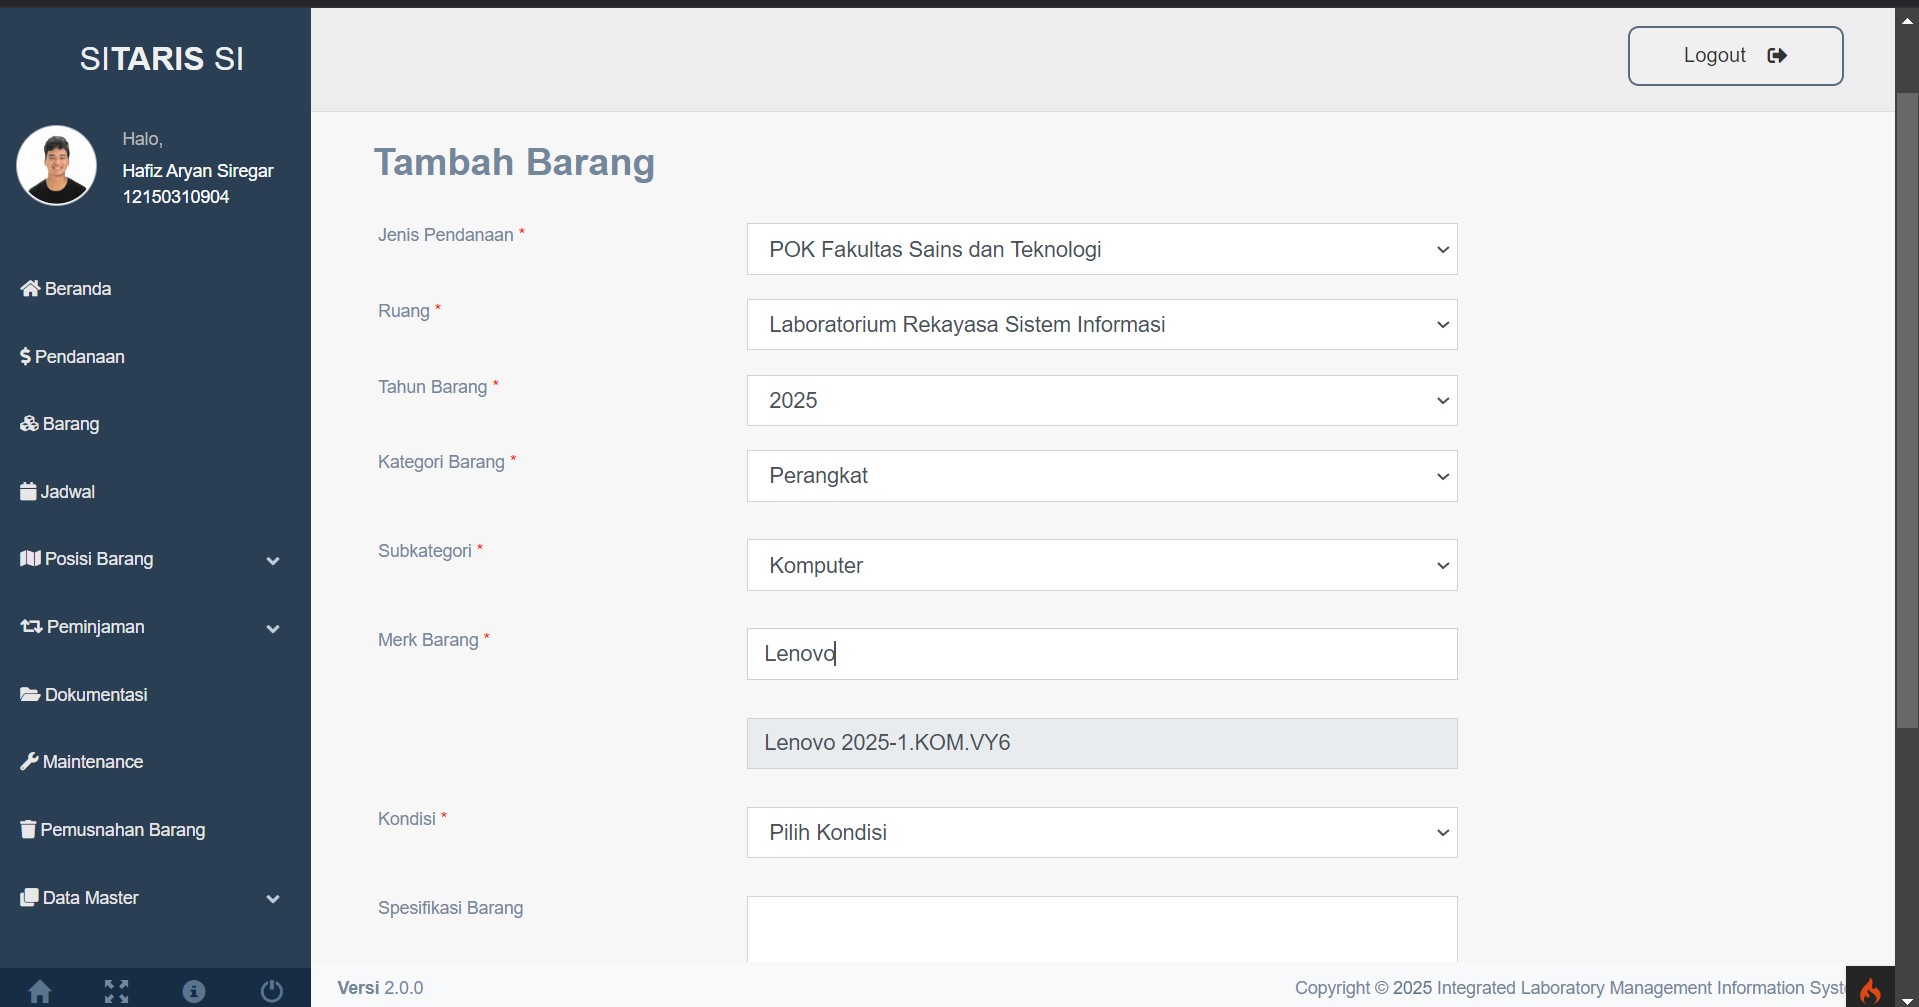
\includegraphics[width=0.82\textwidth]{konten/gambar/perbaikan/kode-barang.png}
		      \caption{Tampilan Kode Barang Sistem Manajemen Laboratorium}
		      \label{fig:kode-barang}
	      \end{figure}

	\item Tampilan pilihan peminjaman yang memungkinkan pengguna memilih jenis peminjaman yang ingin dilakukan. Tampilan ini dirancang untuk memudahkan pengguna dalam menentukan pilihan peminjaman yang sesuai dengan kebutuhan mereka, dengan menyediakan opsi yang jelas dan terstruktur. Dapat dilihat pada Lampiran \ref{fig:pilih-peminjaman}.


	\item Tampilan untuk pengelolaan peminjaman barang yang memudahkan pengguna dalam mengatur dan melihat status peminjaman barang. Tampilan ini menyediakan fitur untuk menambah data peminjaman, serta menampilkan informasi peminjaman dalam format yang mudah dibaca. Dapat dilihat pada Lampiran \ref{fig:peminjaman-barang}.

	\item Tampilan untuk pengelolaan peminjaman ruangan yang memungkinkan pengguna menambah data peminjaman ruangan ke dalam sistem. Tampilan ini dilengkapi dengan form input yang intuitif, sehingga pengguna dapat dengan mudah memasukkan detail peminjaman seperti waktu, tanggal, dan deskripsi kegiatan. Dapat dilihat pada Lampiran \ref{fig:peminjaman-ruangan}.

	\item Tampilan untuk memilih peminjam yang memungkinkan pengguna menentukan peminjam yang akan melakukan peminjaman. Tampilan ini dilengkapi dengan daftar peminjam antara internal maupun eksternal, sehingga pengguna dapat dengan mudah memilih peminjam yang sesuai. Dapat dilihat pada Lampiran \ref{fig:pilih-peminjam}.

\end{enumerate}

Hasil implementasi \textit{interface} berfungsi untuk menunjukkan desain program sistem informasi manajemen laboratorium yang telah dilakukan penambahan. Hal ini dilakukan untuk mempermudah pengguna dalam memahami proses yang terdapat pada sistem informasi manajemen laboratorium tersebut.

\begin{enumerate}
	\item Tampilan \textit{landing page} yang berfungsi sebagai halaman pertama dari sistem informasi manajemen laboratorium. Halaman ini memberikan gambaran umum dan akses awal ke fitur-fitur sistem, serta menyambut pengguna dengan antarmuka yang ramah dan informatif. Dapat dilihat pada Lampiran \ref{fig:landing-page}.

	\item Tampilan pilihan aplikasi untuk \textit{login} yang memungkinkan pengguna memilih aplikasi yang ingin diakses. Tampilan ini dirancang untuk memudahkan pengguna dalam menentukan aplikasi mana yang sesuai dengan kebutuhan mereka, dengan menyediakan opsi yang jelas dan terstruktur. Dapat dilihat pada Lampiran \ref{fig:pilih-login}.

	\item Tampilan kalender laboratorium yang menyajikan jadwal kegiatan laboratorium secara visual dan interaktif. Tampilan ini memungkinkan pengguna untuk melihat jadwal berdasarkan periode waktu tertentu, dengan fitur navigasi bulan dan tahun. Pengguna dapat dengan mudah menambahkan, mengedit, atau menghapus jadwal langsung melalui antarmuka kalender yang responsif. Dapat dilihat pada Lampiran \ref{fig:kalender}.

	\item Tampilan untuk mengelola jadwal laboratorium yang memudahkan pengguna dalam mengatur dan melihat jadwal kegiatan laboratorium. Tampilan ini menyediakan fitur untuk menambah, mengedit, dan menghapus jadwal serta menampilkan jadwal dalam format yang mudah dibaca. Dapat dilihat pada Lampiran \ref{fig:jadwal-keseluruhan} sampai Lampiran \ref{fig:jadwal-int}.

	\item Tampilan untuk menambah jadwal laboratorium yang memungkinkan pengguna menambahkan jadwal baru ke dalam sistem. Tampilan ini dilengkapi dengan form input yang intuitif, sehingga pengguna dapat dengan mudah memasukkan detail jadwal seperti waktu, tanggal, dan deskripsi kegiatan. Dapat dilihat pada Lampiran \ref{fig:tambah-jadwal}.

	\item Tampilan untuk mengedit jadwal laboratorium yang memudahkan pengguna dalam melakukan perubahan pada jadwal yang sudah ada. Tampilan ini menyediakan fitur untuk memperbarui informasi jadwal dengan cepat dan efisien, serta memastikan bahwa semua perubahan tersimpan dengan baik. Dapat dilihat pada Lampiran \ref{fig:edit-jadwal}.

	\item Tampilan untuk mencetak jadwal laboratorium dalam format PDF yang memudahkan pengguna untuk menyimpan dan membagikan jadwal dalam bentuk dokumen digital. Tampilan ini menyediakan fitur untuk mengonversi jadwal yang ada menjadi file PDF dengan cepat dan efisien. Dapat dilihat pada Lampiran \ref{fig:cetak-jadwal}.

	\item Tampilan untuk mengelola mata kuliah laboratorium yang memungkinkan pengguna mengatur mata kuliah yang terkait dengan laboratorium. Tampilan ini menampilkan daftar mata kuliah yang dapat diakses dan dikelola, serta menyediakan opsi untuk menambah atau menghapus mata kuliah sesuai kebutuhan. Dapat dilihat pada Lampiran \ref{fig:matkul}.

	\item Tampilan untuk menambah mata kuliah yang memudahkan pengguna dalam menambahkan mata kuliah baru ke dalam sistem. Tampilan ini menyediakan form input yang lengkap untuk memasukkan informasi mata kuliah seperti nama, kode, dan deskripsi. Dapat dilihat pada Lampiran \ref{fig:tambah-matkul}.

	\item Tampilan untuk mengedit mata kuliah laboratorium yang memungkinkan pengguna melakukan perubahan pada mata kuliah yang sudah ada. Tampilan ini dirancang untuk memudahkan pengguna dalam memperbarui informasi mata kuliah dengan cepat dan akurat. Dapat dilihat pada Lampiran \ref{fig:edit-matkul}.

	\item Tampilan untuk mengelola dosen laboratorium yang memudahkan pengguna dalam mengatur data dosen yang terkait dengan laboratorium. Tampilan ini menampilkan daftar dosen yang terdaftar dan menyediakan fitur untuk menambah, mengedit, atau menghapus data dosen. Dapat dilihat pada Lampiran \ref{fig:dosen}.

	\item Tampilan untuk menambah dosen laboratorium yang memungkinkan pengguna menambahkan data dosen baru ke dalam sistem. Tampilan ini dilengkapi dengan form input yang memudahkan pengguna dalam memasukkan informasi dosen seperti nama, NIDN, dan bidang keahlian. Dapat dilihat pada Lampiran \ref{fig:tambah-dosen}.

	\item Tampilan untuk mengedit dosen laboratorium yang memudahkan pengguna dalam melakukan perubahan pada data dosen yang sudah ada. Tampilan ini menyediakan fitur untuk memperbarui informasi dosen dengan mudah dan memastikan bahwa data yang tersimpan selalu akurat dan terkini. Dapat dilihat pada Lampiran \ref{fig:edit-dosen}.

\end{enumerate}

\section{Pengujian Sistem}
Metode \textit{Black box} digunakan untuk menguji fitur-fitur yang ada pada sistem. Pengujian ini dilakukan untuk memastikan bahwa setiap fungsi dalam sistem berjalan sesuai dengan spesifikasi yang telah ditentukan. Metode ini hanya berfokus pada pengujian keluaran sistem berdasarkan masukan tertentu, tanpa memperhatikan proses internal atau struktur kode.

Pada pengujian Metode \textit{Black box}, peneliti melakukan pengujian terhadap fitur-fitur yang ada pada sistem. Pengujian ini dilakukan oleh peneliti dan beberapa pengguna seperti Aslab dan Admin untuk memastikan bahwa fitur-fitur yang ada pada sistem berjalan dengan baik. Pengujian ini dapat dilihat pada Tabel~\ref{tab:PengujianBlackBox}.

{\fontsize{11pt}{13pt}\selectfont
\begin{longtable}{p{0.01\linewidth} p{0.15\linewidth} p{0.3\linewidth} p{0.3\linewidth} p{0.1\linewidth}}
	\caption{Pengujian \textit{Black box}}\label{tab:PengujianBlackBox}                                                                                                                                              \\
	\hline
	\textbf{No}    & \textbf{Fitur}            & \textbf{Hasil yang diharapkan}                                  & \textbf{Hasil Pengujian}                                                        & \textbf{Status} \\ \hline
	\endfirsthead
	\caption[]{Pengujian \textit{Black box} (Tabel lanjutan...)}                                                                                                                                                     \\
	\hline
	\textbf{No}    & \textbf{Fitur}            & \textbf{Hasil yang diharapkan}                                  & \textbf{Hasil Pengujian}                                                        & \textbf{Status} \\ \hline
	\endhead
	\endfoot
	\endlastfoot
	\centering 1   & Registrasi                & Berhasil melakukan registrasi akun                              & Admin dapat melakukan registrasi akun untuk Kalab, Kaprodi, Sekprodi, dan Aslab & Berhasil        \\
	\centering 2   & \textit{Login} Umum       & Berhasil melakukan \textit{login} dan masuk ke dalam sistem     & Pengguna dapat melakukan \textit{login} ke dalam sistem                         & Berhasil        \\
	\centering 3   & \textit{Login} ke SITARIS & Berhasil masuk ke dalam sistem SITARIS                          & Pengguna dapat melakukan \textit{login} ke dalam sistem SITARIS                 & Berhasil        \\
	\centering  4  & \textit{Login} ke LABVIS  & Berhasil masuk ke dalam sistem LABVIS                           & Pengguna dapat melakukan \textit{login} ke dalam sistem LABVIS                  & Berhasil        \\
	\centering   5 & \textit{Login} ke LARIS   & Berhasil masuk ke dalam sistem LARIS                            & Pengguna dapat melakukan \textit{login} ke dalam sistem LARIS                   & Berhasil        \\
	\centering 6   & Profil                    & Berhasil melakukan perubahan informasi pribadi                  & Pengguna dapat melakukan perubahan informasi pribadi                            & Berhasil        \\
	\centering 7   & Tambah Jadwal             & Berhasil menambah Jadwal                                        & Pengguna berhasil menambah Jadwal                                               & Berhasil        \\
	\centering 8   & Detail Jadwal             & Berhasil melihat detail informasi jadwal                        & Pengguna dapat melihat seluruh informasi jadwal                                 & Berhasil        \\
	\centering 9   & Edit Jadwal               & Berhasil melakukan perubahan status seleksi administrasi jadwal & Pengguna dapat melakukan perubahan status seleksi administrasi jadwal           & Berhasil        \\
	\centering 10  & Hapus Jadwal              & Berhasil menghapus jadwal                                       & Pengguna dapat menghapus jadwal yang sudah terdaftar di sistem                  & Berhasil        \\
	\centering 11  & Cetak Jadwal              & Berhasil mencetak jadwal dalam bentuk PDF                       & Pengguna berhasil mencetak dan \textit{mendownload} jadwal dalam bentuk PDF     & Berhasil        \\
	\centering 12  & Tambah Dosen              & Berhasil menambah Dosen                                         & Pengguna berhasil menambah Dosen                                                & Berhasil        \\
	\centering 13  & Detail Dosen              & Berhasil melihat detail informasi Dosen                         & Pengguna dapat melihat seluruh informasi Dosen                                  & Berhasil        \\
	\centering 14  & \textit{Edit} Dosen       & Berhasil melakukan perubahan status seleksi administrasi Dosen  & Pengguna dapat melakukan perubahan status seleksi administrasi Dosen            & Berhasil        \\
	\centering 15  & Hapus Dosen               & Berhasil menghapus Dosen                                        & Pengguna dapat menghapus Dosen yang sudah terdaftar di sistem                   & Berhasil        \\
	\centering 16  & Tambah Mata Kuliah        & Berhasil menambahkan mata kuliah                                & Dapat menambahkan mata kuliah                                                   & Berhasil        \\
	\centering 17  & \textit{Edit} Mata Kuliah & Berhasil melakukan perubahan mata kuliah                        & Dapat melakukan perubahan terhadap mata kuliah                                  & Berhasil        \\
	\centering 18  & Hapus Mata Kuliah         & Berhasil menghapus mata kuliah                                  & Dapat menghapus mata kuliah                                                     & Berhasil        \\
	\centering 19  & Ubah \textit{password}    & Berhasil melakukan perubahan \textit{password}                  & Pengguna dapat melakukan perubahan \textit{password}                            & Berhasil        \\
	\centering 20  & \textit{Logout}           & Berhasil melakukan \textit{logout}                              & Pengguna dapat keluar dari sistem                                               & Berhasil        \\ \hline
\end{longtable}
}

